\documentclass{sprawozdanie-agh}

\usepackage[utf8]{inputenc}
\usepackage{listings}
\usepackage{xcolor}
\usepackage{graphicx}
\usepackage{caption}
\usepackage{graphicx}
\usepackage{wrapfig}
\usepackage{subcaption}
\usepackage{accsupp}
\usepackage{array}
\usepackage{amsfonts}
\usepackage[shortlabels]{enumitem}
\usepackage{amsmath, xparse}
\usepackage{listings}
\usepackage{booktabs}

\graphicspath{ {./img/} }

\makeatletter

\begin{document}

\przedmiot{Algorytmy geometryczne}
\tytul{Laboratorium 2}
\podtytul{Otoczka wypukła}
\kierunek{Informatyka}
\autor{Kyrylo Iakymenko}
\data{Kraków, 7 listopada 2023}

\stronatytulowa{}

\section{Wprowadzenie}
\subsection{Cel ćwiczenia}
\quad To ćwiczenie ma na celu zapoznanie się z metodami generacji 
losowych punktów oraz badanie metod klasyfikacji położenia punktów na płaszczyźnie 
względem prostej. 
\subsection{Położenie punktu względem prostej}

\quad Położenie punktu względem prostej będziemy wyznaczać obliczjąc
dane wyznaczniki. Wyznaczniki pozwalają określić położenie
punktu c względem prostej która jest wyznaczona przez punkty a i b.
Jeżeli wyznacznik jest większy od 0 to punkt znajduje się z lewej strony prostej, jeżeli jest mniejszy
od 0  to
punkt znajduje się po prawej stronie prostej, a jeżeli wartość wyznacznika
jest równa 0 (lub jej wartość bezwzględna $< \varepsilon$) to punkt leży na prostej.

\quad Pomimo, że
powyższe wyznaczniki są sobie równoważne to na skutek
niedoskonałości reprezentacji liczb rzeczywistych w komputerze wyniki
mogą się różnić w zależności od użytego wyznacznika.

$$
(1)\det(a, b, c)= \begin{vmatrix}
       a_{x} - c_{x} & a_{y} - c_{y} \\
       b_{x} - c_{x} & b_{y} - c_{y} 
              \end{vmatrix}.\\
              $$
              $$
(2)\det(a, b, c) = \begin{vmatrix}
    a_x & a_y & 1\\
    b_x & b_y & 1\\
    c_x & c_y & 1
\end{vmatrix}.\\
$$
\section{Opis wykorzystanych algorytmów}
\subsection{Algorytm Grahama}

\quad Algorytm Grahama jest popularnym algorytmem do wyznaczania otoczki wypukłej dla zbioru punktów w przestrzeni dwuwymiarowej. Ten algorytm jest bardziej efektywny niż algorytm Jarvisa i ma złożoność czasową wynoszącą $O(nlog(n))$, gdzie $n$ to liczba punktów w zbiorze. Algorytm Grahama opiera się na wykorzystaniu sortowania punktów względem ich kąta względem punktu startowego.

Poniżej przedstawiam kroki algorytmu Grahama:

Wybieramy punkt startowy, który będzie częścią otoczki wypukłej. W praktyce często wybiera się punkt o najniższej wartości współrzędnej y (jeśli istnieje więcej niż jeden taki punkt, wybiera się ten z najniższą wartością współrzędnej x).

Sortujemy pozostałe punkty ze zbioru według kąta, jaki tworzą względem punktu startowego. Dzięki temu punkty są rozmieszczone w kolejności od najmniejszego kąta do największego kąta. W przypadku, gdy wiele punktów ma ten sam kąt, sortowane są względem odległości od punktu startowego.

Algorytm przetwarza punkty w kolejności rosnących kątów. Początkowo dodajemy punkt startowy do otoczki wypukłej.

Dla każdego punktu, który przetwarzamy, sprawdzamy, czy tworzy on odcinek wypukły w stosunku do ostatnich dwóch punktów na otoczce. Jeśli tak, dodajemy ten punkt do otoczki wypukłej.

Jeśli punkt nie tworzy odcinka wypukłego, to usuwamy ostatni punkt otoczki i sprawdzamy punkt obecny ponownie w kontekście poprzedniego punktu na otoczce.

Algorytm kończy działanie, gdy wszystkie punkty zostały przetworzone, a otoczka wypukła została zakończona.






\subsection{Algorytm Jarvisa}
\quad Algorytm Jarvisa, znany również jako algorytm "Gift Wrapping", to jedna metod wyznaczania otoczki wypukłej dla zbioru punktów w przestrzeni dwuwymiarowej. Ten algorytm jest stosunkowo prosty w implementacji, choć ma złożoność czasową wynoszącą $O(nh)$, gdzie $n$ to liczba punktów w zbiorze, a $h$ to liczba punktów na otoczce wypukłej.

Poniżej przedstawiam kroki algorytmu Jarvisa:

Na początek należy wybrać punkt startowy, który będzie częścią otoczki wypukłej. Często wybiera się punkt o najniższej wartości współrzędnej y (jeśli istnieje więcej niż jeden taki punkt, wybiera się ten z najniższą wartością współrzędnej x).

Ustalamy punkt startowy jako pierwszy punkt otoczki wypukłej.

W kolejnej fazie algorytmu próbujemy znaleźć punkt z otoczki, który znajduje się na prawo od odcinka łączącego bieżący punkt otoczki z poprzednim punktem otoczki. To oznacza, że nowy punkt musi tworzyć odcinek wypukły w stosunku do bieżącej otoczki.

Algorytm działa w pętli, w której znajduje się następny punkt otoczki, który spełnia kryterium odcinka wypukłego, aż wróci do punktu początkowego, co oznacza, że otoczka została zamknięta.

Po znalezieniu kolejnego punktu, dodajemy go do otoczki wypukłej.

Algorytm kończy działanie, gdy wróci do punktu początkowego, tworząc zamkniętą otoczkę wypukłą.

\section{Generowanie zbiorów punktów}
\quad Na potrzeby ćwiczenia wygenerujemy $4$ zbiory punktów losowych.
\begin{enumerate}[a)]
    \item Losowe punkty $(x, y)$ w przestrzeni $\mathbb{R}^2$, gdzie $(x, y) \in \left[-10^4,10^4\right]^{2}$.
    \item Losowe punkty $(x, y)$ w przestrzeni $\mathbb{R}^2$, położone na okręgu o promieniu $R = 10^4$.
    \item Losowe punkty w przestrzeni $\mathbb{R}^2$, 
    położone na prostokącie o wierzcholku w $(-10^4, -10^4)$ i $(10^4, 10^4)$.
    \item Losowe punkty w przestrzeni $\mathbb{R}^2$, 
    położone na dolnym i lewym bokack kwadratu o wierzcholku w $(-10^4, -10^4)$ i $(10^4, 10^4)$ i jego przekątnych.
\end{enumerate}

\subsection{Wykresy zbiorów}
\begin{figure}[!h]
    \centering
    \begin{subfigure}{.5\textwidth}
      \centering
      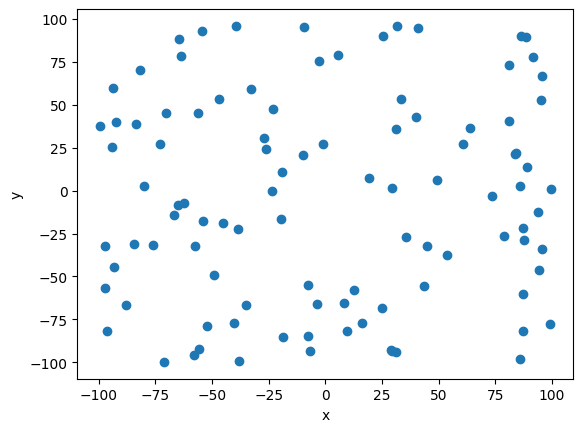
\includegraphics[width=.9\linewidth]{a.png}
      \caption*{Rys. 1: Zbiór $a$.}
      \label{fig:sub1}
    \end{subfigure}%
    \begin{subfigure}{.5\textwidth}
      \centering
      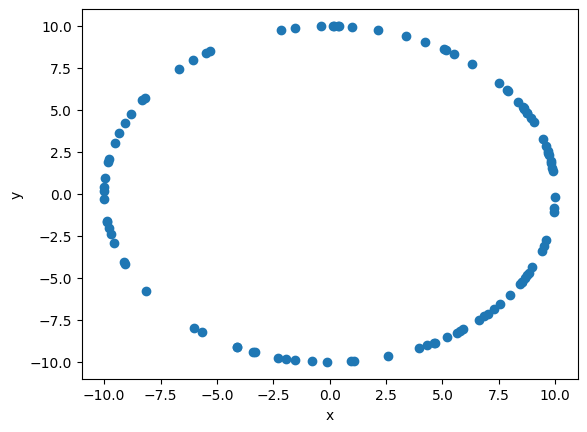
\includegraphics[width=.9\linewidth]{b.png}
      \caption*{Rys. 2: Zbiór $b$.}
      \label{fig:sub2}
    \end{subfigure}
    \label{fig:test}
    \end{figure}
    \begin{figure}[!h]
    \centering
    \begin{minipage}{.5\textwidth}
      \centering
      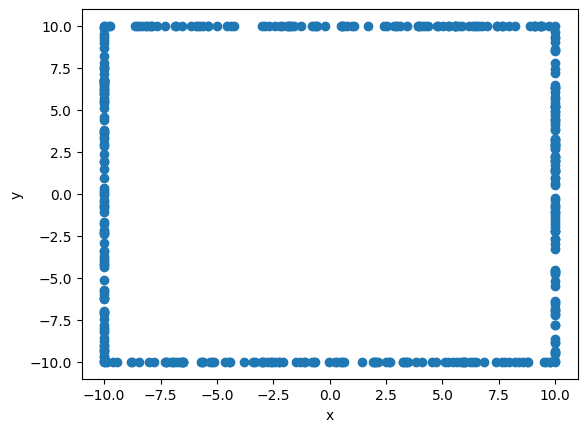
\includegraphics[width=.9\linewidth]{c.png}
      \caption*{Rys. 3: Zbiór $c$.}
      \label{fig:test1}
    \end{minipage}%
    \begin{minipage}{.5\textwidth}
      \centering
      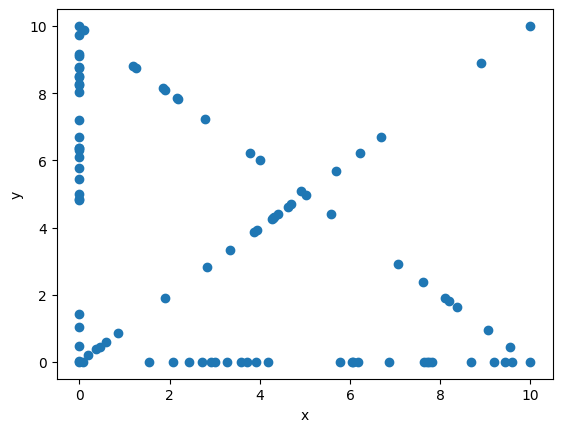
\includegraphics[width=.9\linewidth]{d.png}
      \caption*{Rys. 4: Zbiór $d$.}
      \label{fig:test2}
    \end{minipage}
    \end{figure}
\null
    \subsection{Algorytmy generacji zbiorów}
    \begin{enumerate}
    \item Dla zbioru a. Osobna generacja każdego z lososwych punktów.
    \item Dla zbioru b. Parametryzacja punktów na okręgu za pomocją funkcji trygonometrycznych $\sin$ i $\cos$.
    \item Dla zbioru c. Parametryzacja punktów na okręgu za pomocją funkcji trygonometrycznych $\sin$ i $\cos$.
    \item Dla zbioru d. Przekształcenie odcinka do postaci parametrycznej 
    $$
    l:\begin{cases}
      x = x_0 + tv_x& \smash{\raisebox{-1.6ex}{dla $\boldsymbol t \in [0,1]$.}}\\
      y = y_0 + tv_y
    \end{cases}
    $$
    A potem generowanie $t$ w podanym przedziale i dodanie odpowiednich punktów.
    \end{enumerate}
% \newpage

\section{Wydajność algorytmów}
\subsection{Opis zbiorów testowych}
\quad Na potrzeby pomiarów wydajności obu algorytmów zmodyfikujemy nasze zbiory testowe 
opisane wyżej w następujący sposób.
\begin{enumerate}[a)]
    \item Losowe punkty $(x, y)$ w przestrzeni $\mathbb{R}^2$, gdzie $(x, y) \in \left[-10^4,10^4\right]^{2}$.
    \item Losowe punkty $(x, y)$ w przestrzeni $\mathbb{R}^2$, położone na okręgu o promieniu $R = 10^4$.
    \item Losowe punkty w przestrzeni $\mathbb{R}^2$, 
    położone na prostokącie o wierzcholku w $(-10^4, -10^4)$ i $(10^4, 10^4)$.
    \item Losowe punkty w przestrzeni $\mathbb{R}^2$, 
    położone na dolnym i lewym bokack kwadratu o wierzcholku w $(-10^4, -10^4)$ i $(10^4, 10^4)$ i jego przekątnych.
\end{enumerate}

\subsection{Tabele}
\quad Czasy wykonania algorytmów na zbiorach testowych w zależności od ilości punktów podane w sekundach $[s]$.
\renewcommand{\arraystretch}{2}
\begin{table}[!ht]
    \centering
\begin{tabular}{l  c|c|c|c|}
    & \multicolumn{4}{c}{\textbf{Liczba punktów}} \\ \cline{2-5}     
    \multicolumn{1}{l|}{\textbf{Algorytm}} & $10^3$& $10^4$& $10^5$& $10^6$ \\
   \hline
   \hline
   \multicolumn{1}{l|}{\textbf{Graham}} & 0.007& 0.088& 1.222& 15.013 \\
   \hline
   \multicolumn{1}{l|}{\textbf{Jarvis}} & 0.010& 0.107& 1.771& 25.266 \\
   \cline{2-5}
\end{tabular}
\caption*{Tabela 1: Czasy wykonania algorytmów na zbiorze testowym $a$.}
\end{table}


\begin{table}[!ht]
    \centering
\begin{tabular}{l  c|c|c|}
    & \multicolumn{3}{c}{\textbf{Liczba punktów}} \\ \cline{2-4}     
    \multicolumn{1}{l|}{\textbf{Algorytm}} & 100& $10^3$& $10^4$ \\
   \hline
   \hline
   \multicolumn{1}{l|}{\textbf{Graham}} & 0.001& 0.011& 0.130 \\
   \hline
   \multicolumn{1}{l|}{\textbf{Jarvis}} & 0.008& 0.678& 70.709 \\
   \cline{2-4}
\end{tabular}
\caption*{Tabela 2: Czasy wykonania algorytmów na zbiorze testowym $b$.}
\end{table}

\newpage
\begin{table}[!ht]
    \centering
\begin{tabular}{l  c|c|c|c|c|}
    & \multicolumn{5}{c}{\textbf{Liczba punktów}} \\ \cline{2-6}     
    \multicolumn{1}{l|}{\textbf{Algorytm}} & 100& $10^3$& $10^4$& $10^5$& $10^6$ \\
   \hline
   \hline
   \multicolumn{1}{l|}{\textbf{Graham}} & 0.005& 0.064& 0.739& 9.177& 113.494 \\
   \hline
   \multicolumn{1}{l|}{\textbf{Jarvis}} & 0.001& 0.009& 0.115& 1.242& 13.464 \\
   \cline{2-6}
\end{tabular}
\caption*{Tabela 3: Czasy wykonania algorytmów na zbiorze testowym $c$.}
\end{table}


\begin{table}[!ht]
    \centering
\begin{tabular}{l  c|c|c|c|c|}
    & \multicolumn{5}{c}{\textbf{Liczba punktów}} \\ \cline{2-6}     
    \multicolumn{1}{l|}{\textbf{Algorytm}} & 100& $10^3$& $10^4$& $10^5$& $10^6$ \\
   \hline
   \hline
   \multicolumn{1}{l|}{\textbf{Graham}} & 0.002& 0.027& 0.212& 2.816& 37.919 \\
   \hline
   \multicolumn{1}{l|}{\textbf{Jarvis}} & 0.001& 0.011& 0.077& 0.921& 9.709 \\
   \cline{2-6}
\end{tabular}
\caption*{Tabela 4: Czasy wykonania algorytmów na zbiorze testowym $d$.}
\end{table}


\section{Opracowanie wyników}
\section{Podsumowanie}
W trakcie prowadzenia tego badania przeprowadziliśmy analizę i porównanie dwóch popularnych algorytmów służących do wyznaczania otoczki wypukłej, tj. algorytmów Grahama i Jarvisa. Naszym celem było zrozumienie działania tych algorytmów oraz porównanie ich wydajności przy użyciu różnych zbiorów punktów. Poniżej przedstawiamy główne wnioski z naszych badań:

Algorytm Grahama:

Algorytm Grahama charakteryzuje się złożonością czasową wynoszącą O(n*log(n)), co sprawia, że jest bardziej wydajny niż algorytm Jarvisa.
Jest efektywny w przypadku zbiorów punktów o większej liczbie elementów, co sprawia, że jest bardziej przydatny w rzeczywistych zastosowaniach.
Algorytm Jarvisa:

Algorytm Jarvisa jest prosty w implementacji, ale jego złożoność czasowa wynosi O(nh), gdzie "n" to liczba punktów, a "h" to liczba punktów na otoczce wypukłej.
Jego wydajność maleje znacząco w przypadku zbiorów punktów o dużym rozmiarze, co sprawia, że może być mniej praktyczny w niektórych sytuacjach.
Porównanie:

W naszych badaniach zaobserwowaliśmy, że algorytm Grahama osiąga lepsze wyniki wydajnościowe niż algorytm Jarvisa, zwłaszcza w przypadku dużych zbiorów punktów.
Algorytm Grahama jest bardziej efektywny dzięki zastosowaniu sortowania punktów względem kąta względem punktu startowego, co pozwala na znaczne przyspieszenie procesu wyznaczania otoczki wypukłej.
Podsumowując, zarówno algorytm Grahama, jak i algorytm Jarvisa znajdują zastosowanie w wyznaczaniu otoczki wypukłej, ale wybór między nimi zależy od konkretnych potrzeb i rozmiaru zbioru punktów. Algorytm Grahama jest bardziej efektywny i zwykle bardziej polecany w praktyce, zwłaszcza w przypadku dużych zbiorów punktów, gdzie złożoność czasowa odgrywa kluczową rolę. Jednak algorytm Jarvisa pozostaje przydatnym narzędziem, zwłaszcza w celach edukacyjnych i w przypadku mniejszych zbiorów punktów, gdzie prostota implementacji może mieć znaczenie.





\end{document}